\documentclass{article}

\usepackage{graphicx} 
\usepackage[margin=0.75in]{geometry}
\usepackage{url}

\begin{document}

\section{Team 4}
\begin{table}[htbp]
  \centering
  \caption{Members}
  \label{tab:team_table}
  \begin{tabular}{| l | c |}
    \hline
    \textbf{Name} & \textbf{Email} \\ \hline
    Jackson Weibel(Team Leader)            & jacksonweibel@tamu.edu                  \\ \hline
    Miles Turnage         & milesturnage@tamu.edu                     \\ \hline
    Gabriel Rangel-Orozco         & gabrielrangelorozco@tamu.edu                     \\ \hline
    Gwilym Couch         & gwilymcouch@tamu.edu                     \\ \hline
    Vihaan Ketavarapu         & vihaanket@tamu.edu                     \\ \hline
  \end{tabular}
\end{table}

\noindent
\textbf{GitHub Repository:}
\url{https://github.com/JacksonWeibelDev/DAEN328-Term-Project}


\section{Data Source}
Our group selected the National Crime Victimization Survey (NVCS) Personal Victimization dataset, published by the Bureau of Justice Statistics.

\begin{itemize}
  \item API: 
  \url{https://api.ojp.gov/bjsdataset/v1/gcuy-rt5g.json}

  \item This is our own proposal.
  \item No api key is needed.
  \item The survey is conducted annually, with historical data from 1993 to 2024.
  \item The API supports pagination using limit and offset parameters.
  \item Each entry has a unique identifier(idper) we will use for incremental pulls.
\end{itemize}

\section{Proof it works}


\begin{figure}[htbp]
    \centering
    % 2. Insert your image file name here (omit the extension like .png/.jpg)
    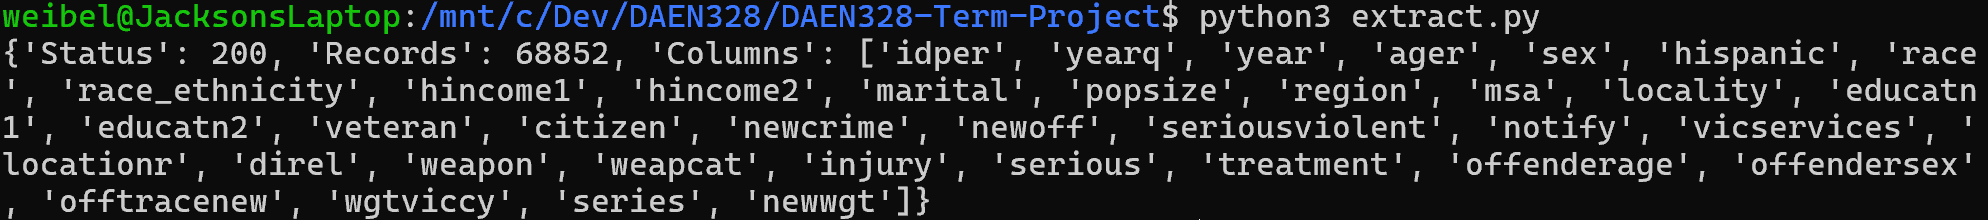
\includegraphics[width=1\linewidth]{ProofItWorks} 
    \caption{Successful NCVS API request returning 68,852 records and 37 columns.}
    \label{fig:proof_it_works_picture} % Used to cross-reference in text
\end{figure}

\section{Data description}
Our project will analyze crime victimization patterns in
the United States, focusing on the relationship between
crime characteristics and whether incidents are reported
to police. The goal is to identify patterns that could
help researchers better understand unreported victimization.

Our dashboard will answer five questions:

\begin{enumerate}
  \item Which types of victimizations are most and least likely to be reported?

  \item How have police reporting patterns changed over time?

  \item How does the victim-offender relationship relate to police reporting?

  \item Are victimizations involving weapons or injuries more frequently reported?

  \item How do reporting patterns differ by age group and region?
\end{enumerate}

Our proposed PostgreSQL tables:

\begin{itemize}
  \item \textbf{Respondents:}
    Stores demographic and background information
    about surveyed individuals.

    \textbf{Columns:}
    \texttt{idper}, \texttt{yearq}, \texttt{year},
    \texttt{ager}, \texttt{sex}, \texttt{hispanic},
    \texttt{race}, \texttt{race\_ethnicity},
    \texttt{hincome1}, \texttt{hincome2},
    \texttt{marital}, \texttt{popsize},
    \texttt{region}, \texttt{msa}, \texttt{locality},
    \texttt{educatn1}, \texttt{educatn2},
    \texttt{veteran}, \texttt{citizen}.

    Proposed composite primary key:
    \texttt{(idper, yearq)}.

  \item \textbf{Offense Types:}
    Stores crime classifications and descriptions.

    \textbf{Columns:}
    \texttt{newoff}, \texttt{newcrime},
    \texttt{seriousviolent}, and
    \texttt{offense\_name} (derived from the codebook).

    Primary key: \texttt{newoff}.

  \item \textbf{Victimizations:}
    Stores individual victimization records,
    including reporting status, crime circumstances,
    offender characteristics, and survey weights.

    \textbf{Columns:}
    \texttt{victimization\_id} (source \texttt{:id}),
    \texttt{idper}, \texttt{yearq}, \texttt{newoff},
    \texttt{notify}, \texttt{vicservices},
    \texttt{locationr}, \texttt{direl},
    \texttt{weapon}, \texttt{weapcat},
    \texttt{injury}, \texttt{serious},
    \texttt{treatment}, \texttt{offenderage},
    \texttt{offendersex}, \texttt{offtracenew},
    \texttt{wgtviccy}, \texttt{series},
    \texttt{newwgt}, \texttt{updated\_at}
    (source \texttt{:updated\_at}).

    Provisional primary key:
    \texttt{victimization\_id}.

    Foreign keys:
    \texttt{(idper, yearq)} references Respondents;
    \texttt{newoff} references Offense Types.
\end{itemize}

\section{Plan and Roles}
\begin{table}[htbp]
  \centering
  \caption{Members}
  \label{tab:team_table}
  \begin{tabular}{| l | c |}
    \hline
    \textbf{Name} & \textbf{Role} \\ \hline
    Jackson Weibel            &  Docker, Loading                \\ \hline
    Miles Turnage         &  Extraction                    \\ \hline
    Gabriel Rangel-Orozco         &     Dashboard                \\ \hline
    Gwilym Couch         &            Shadowing          \\ \hline
    Vihaan Ketavarapu         &        Transformation             \\ \hline
  \end{tabular}
\end{table}

\noindent
\textbf{Project Risk:}
One potential challenge is the dataset's incremental
update behavior. Our tests showed that records from
multiple survey years shared the same update timestamp,
suggesting that BJS may refresh data in bulk.

To address this, we plan to track the last successful
update timestamp, use PostgreSQL UPSERT operations
to prevent duplicate records, and validate record
identifier stability.

\end{document}